## Test ##
\documentclass[a4paper]{article}

%%\usepackage{showframe}
\usepackage{graphicx}
\usepackage{float}

\usepackage[utf8]{inputenc}

\usepackage[useregional]{datetime2}

\usepackage{csquotes}

%\usepackage[T1]{fontenc}
%\renewcommand*\familydefault{\sfdefault} %% Only if the base font of the document is to be sans serif

\usepackage{geometry}
\geometry{
 a4paper,
 left=20mm,
 right=20mm,
 bottom=30mm,
 top=30mm
}

\newcommand{\Version}{1.3.1}

\makeatletter
\title{Standard Setup for NinjaFirewall}\let\Title\@title
\author{Daniel Ruf}\let\Author\@author
\date{2022-02-26} \let\Date\@date
\makeatother

\usepackage[a-1b]{pdfx}
\begin{filecontents*}{\jobname.xmpdata}
  \Title{\Title\ v\Version\ (\Date)}
  \Author{\Author}
  \Language{en-US}
  \Keywords{}
  \Publisher{}
  \Subject{\Title\ v\Version\ (\Date)}
\end{filecontents*}

\usepackage{hyperref}
\hypersetup{
  colorlinks=true,
  linkcolor=blue,
  filecolor=blue,
  urlcolor=blue
}
\urlstyle{same}

\usepackage{fancyhdr}

\pagestyle{fancy}
\fancyhf{}

\begin{document}
\lhead{\Title}
\lfoot{v\Version}
\rfoot{\today}

\noindent

%%{\fontfamily{cmss}\selectfont

\noindent
\textbf{Step 1:} install and activate NinjaFirewall

\begin{figure}[H]
  \centering
  \includegraphics[width=0.85\textwidth]{images/1.png}
\end{figure}

\noindent
\textbf{Step 2:} go to NinjaFirewall -- Event Notifications and copy the contact email

\begin{figure}[H]
  \centering
  \includegraphics[width=0.85\textwidth]{images/2.png}
\end{figure}

\noindent
\textbf{Step 3:} go to \href{https://danielruf.github.io/ninjafirewall-config-browser/}{ninjafirewall config browser}

\begin{figure}[H]
  \centering
  \includegraphics[width=0.85\textwidth]{images/3.png}
\end{figure}

\newpage

\noindent
\textbf{Step 4:} insert the contact email and click the download button

\begin{figure}[H]
  \centering
  \includegraphics[width=0.85\textwidth]{images/4.png}
\end{figure}

\noindent
\textbf{Step 5:} go to NinjaFirewall -- Firewall Options

\begin{figure}[H]
  \centering
  \includegraphics[width=0.85\textwidth]{images/5.png}
\end{figure}

\noindent
\textbf{Step 6:} import the downloaded configuration

\begin{figure}[H]
  \centering
  \includegraphics[width=0.85\textwidth]{images/6.png}
\end{figure}

\begin{figure}[H]
  \centering
  \includegraphics[width=0.85\textwidth]{images/7.png}
\end{figure}

\noindent
\textbf{Step 7:} submit the page (in some cases you may have to repeat step 6 and 7)

\begin{figure}[H]
  \centering
  \includegraphics[width=0.85\textwidth]{images/8.png}
\end{figure}

\noindent
\textbf{Step 8:} go to NinjaFirewall -- Event Notifications, now all events should be enabled

\begin{figure}[H]
  \centering
  \includegraphics[width=0.85\textwidth]{images/9.png}
\end{figure}

\newpage

\noindent
\textbf{Step 9:} go to NinjaFirewall -- Dashboard

\begin{figure}[H]
  \centering
  \includegraphics[width=0.85\textwidth]{images/10.png}
\end{figure}

\noindent
\textbf{Step 10:} click on \enquote{Activate Full WAF mode}

\begin{figure}[H]
  \centering
  \includegraphics[width=0.85\textwidth]{images/11.png}
\end{figure}

\noindent
\textbf{Step 11:} submit the page (scroll down to see the button, the default settings should be fine)

\begin{figure}[H]
  \centering
  \includegraphics[width=0.85\textwidth]{images/12.png}
\end{figure}

\noindent
\textbf{Step 12:} NinjaFirewall will create a .user.ini file next to the wp-config.php file

\begin{figure}[H]
  \centering
  \includegraphics[width=0.85\textwidth]{images/13.png}
\end{figure}

\newpage

\noindent
\textbf{Step 13:} after some time the status should be updated (reload the page)

\begin{figure}[H]
  \centering
  \includegraphics[width=0.85\textwidth]{images/14.png}
\end{figure}

\noindent
\textbf{Step 14:} go to NinjaFirewall -- Monitoring

\begin{figure}[H]
  \centering
  \includegraphics[width=0.85\textwidth]{images/15.png}
\end{figure}

\noindent
\textbf{Step 15:} create a snapshot

\begin{figure}[H]
  \centering
  \includegraphics[width=0.85\textwidth]{images/16.png}
\end{figure}

\newpage

\noindent
\textbf{Step 16:} set scan schedule to daily

\begin{figure}[H]
  \centering
  \includegraphics[width=0.85\textwidth]{images/17.png}
\end{figure}

\noindent
\textbf{Step 17:} click the save button

\begin{figure}[H]
  \centering
  \includegraphics[width=0.85\textwidth]{images/18.png}
\end{figure}

\noindent
\textbf{Step 18:} go to File Guard on the same page

\begin{figure}[H]
  \centering
  \includegraphics[width=0.85\textwidth]{images/19.png}
\end{figure}

\noindent
\textbf{Step 19:} enable File Guard and click the save button

\begin{figure}[H]
  \centering
  \includegraphics[width=0.85\textwidth]{images/20.png}
\end{figure}

\newpage

\noindent
\textbf{Step 20:} open a new incognito window and open your-domain/wp-content/index.php?f=\%00,
the request should be blocked and there should be the following information from NinjaFirewall
which includes the event ID at the bottom
%%\indent bottom.

\begin{figure}[H]
  \centering
  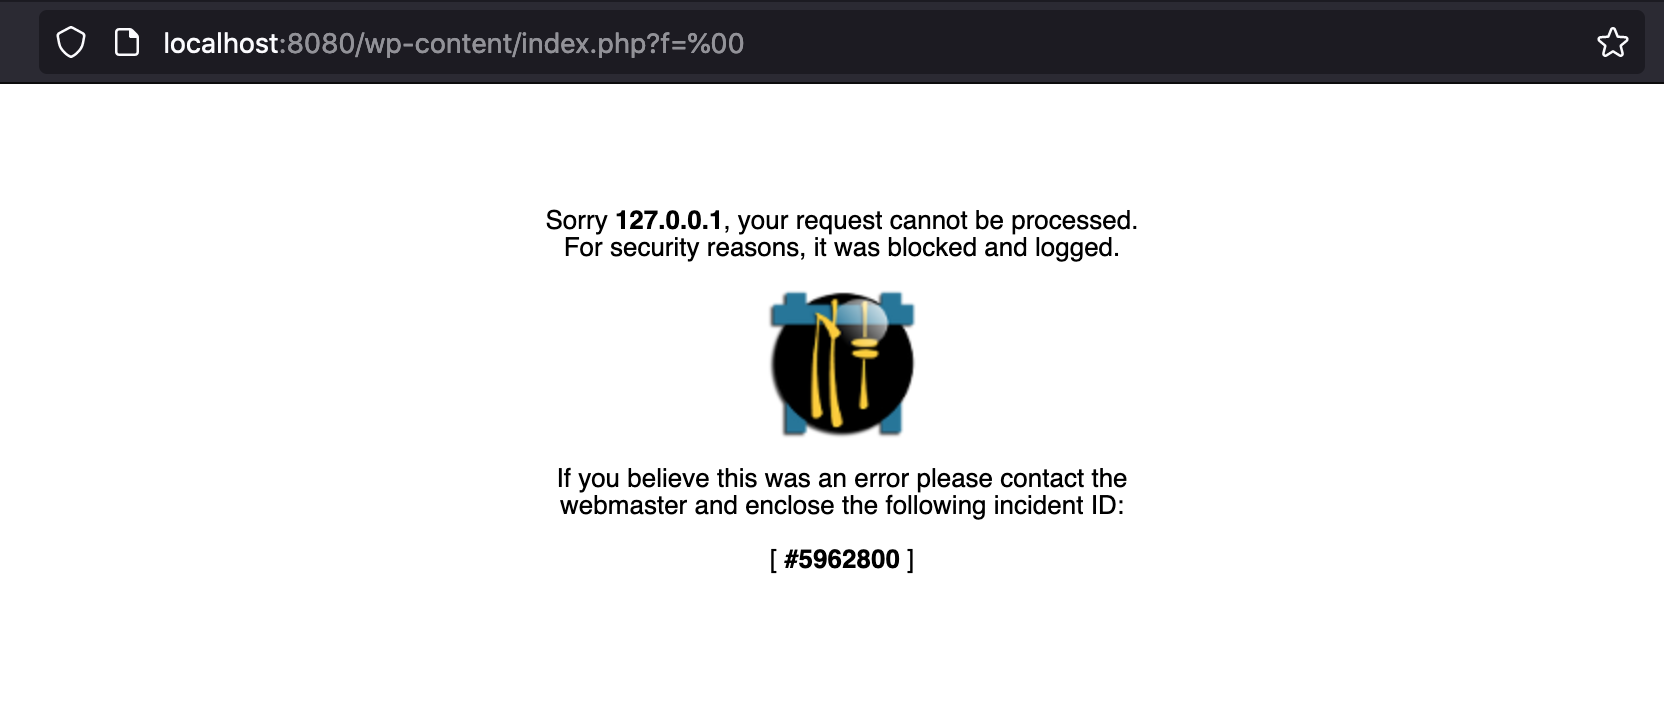
\includegraphics[width=0.85\textwidth]{images/21.png}
\end{figure}

\noindent
\textbf{Step 21:} go to NinjaFirewall -- Logs, the blocked request should now appear there

\begin{figure}[H]
  \centering
  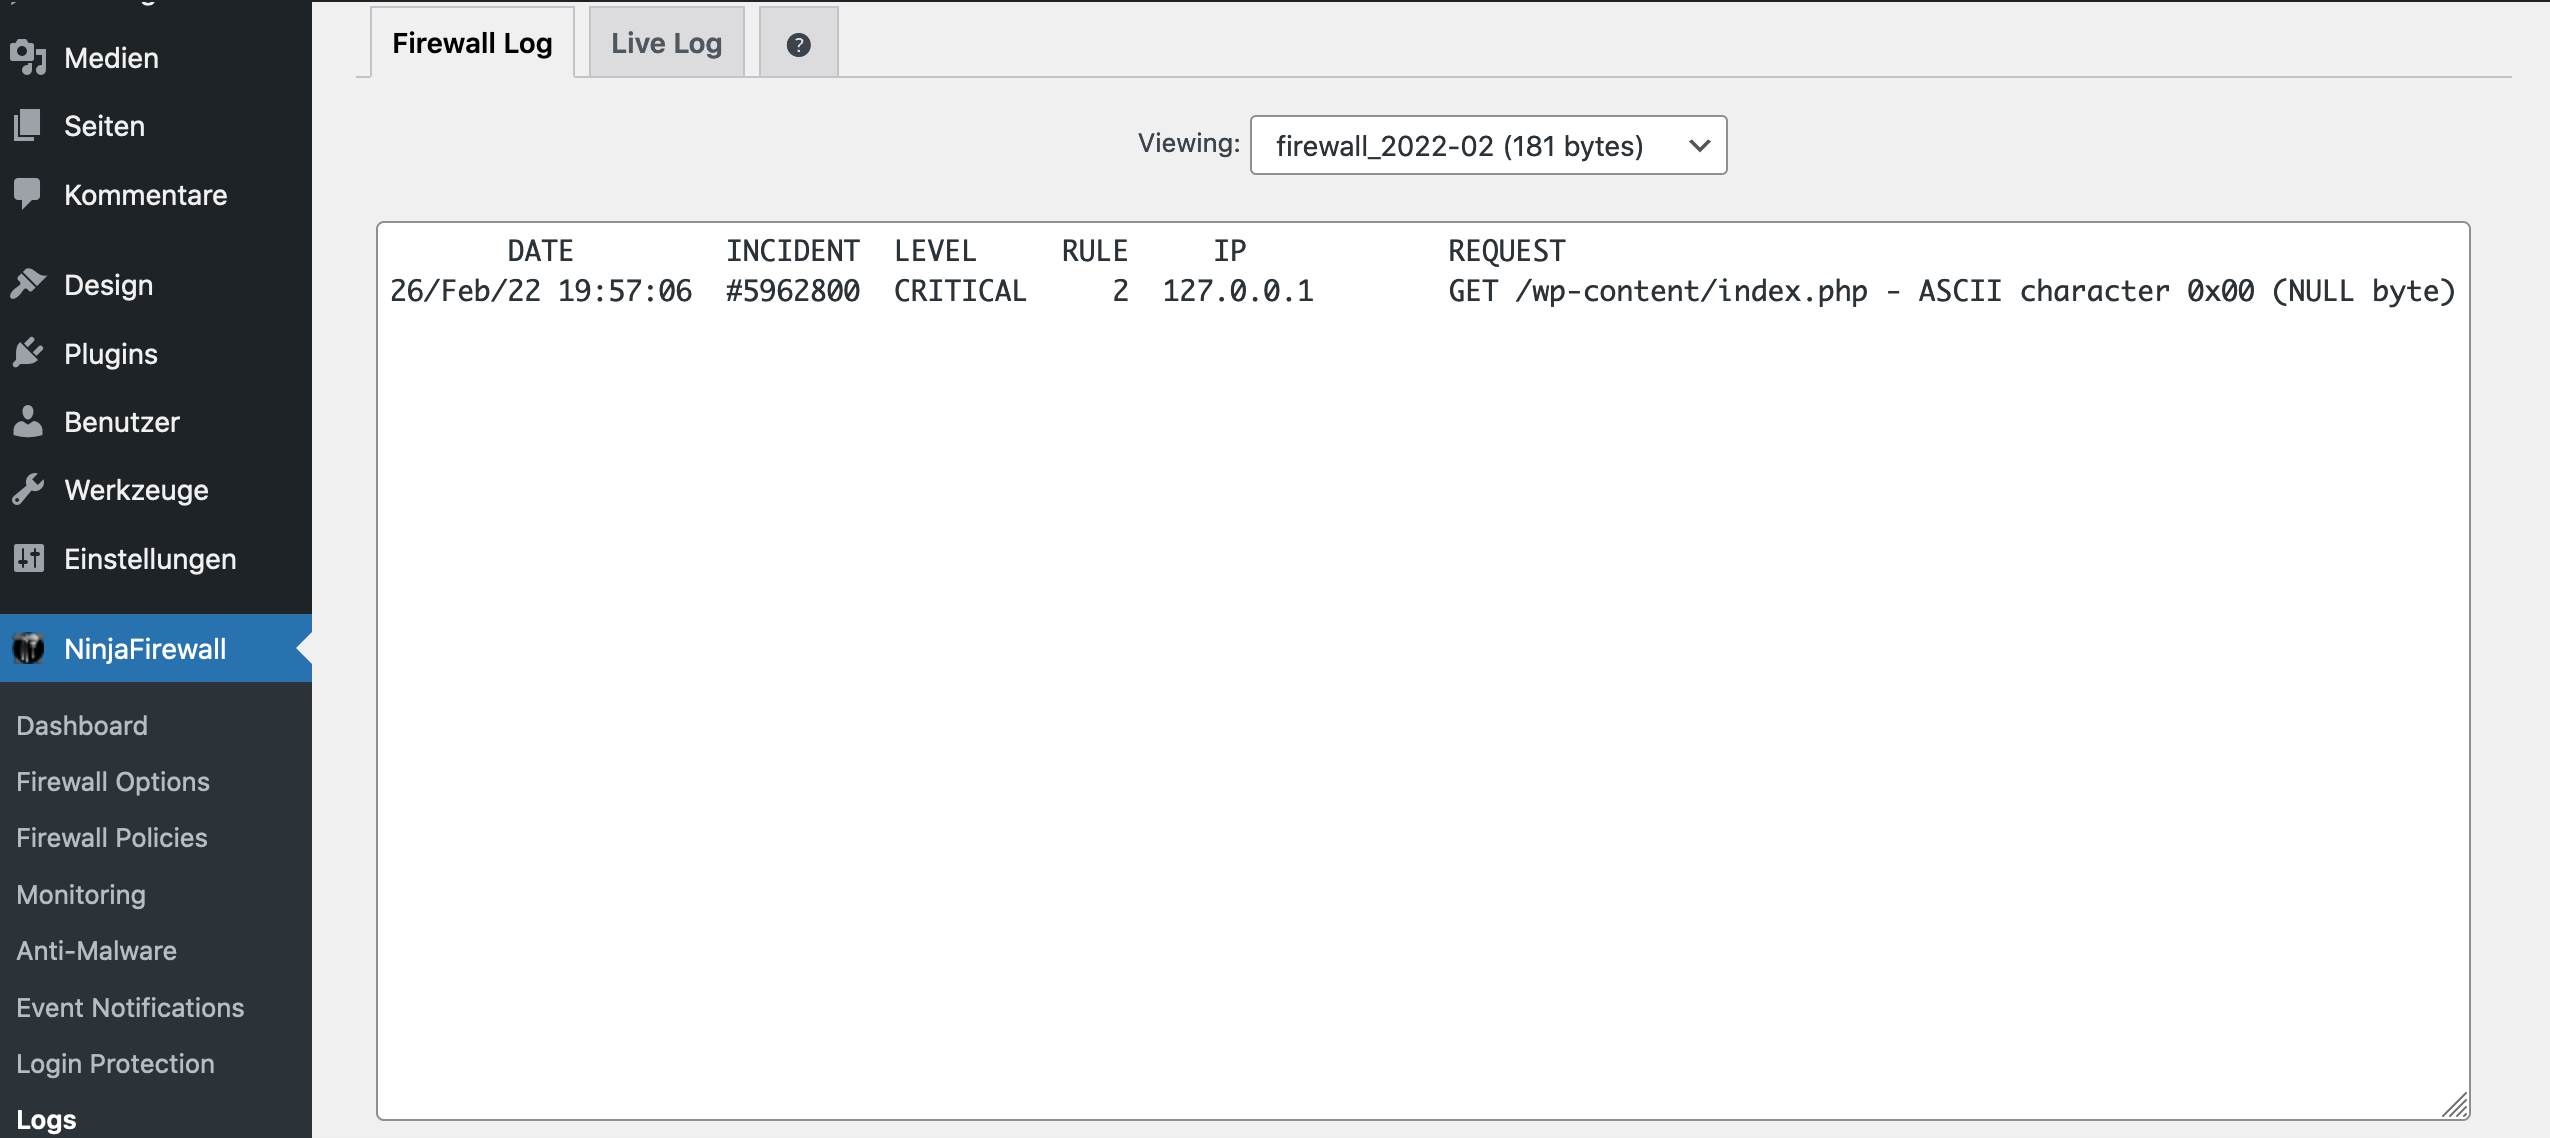
\includegraphics[width=0.85\textwidth]{images/22.png}
\end{figure}

\newpage

\noindent
\textbf{Step 22 (optional):} go to NinjaFirewall -- Login Protection and use the following settings

\begin{figure}[H]
  \centering
  \includegraphics[width=0.85\textwidth]{images/23.png}
\end{figure}

%%}

\end{document}
